% Figure 1 of the week-06 Oscars handout: the Actor in a Leading Role card
% (oscars_card.png, a 2x capture) with numbered markers. Build with
% `make figures` in handouts/, which writes oscars_card_annotated.pdf (for
% the PDF handout) and oscars_card_annotated.png (for the notebook).
% Coordinates are pixels of oscars_card.png, measured in the live page.
\documentclass[border=0pt]{standalone}
\makeatletter\def\input@path{{../../common/}{handouts/common/}}\makeatother
\usepackage[scaled=0.92]{helvet}
\usepackage{graphicx}
\usepackage{handoutmarkers}
\begin{document}
\setlength{\unitlength}{0.002215in}% 1 px; the figure is 2.625in wide in the handout
\begin{tikzpicture}[x=\unitlength,y=-\unitlength]
  \node[anchor=north west,inner sep=0] at (0,0)
    {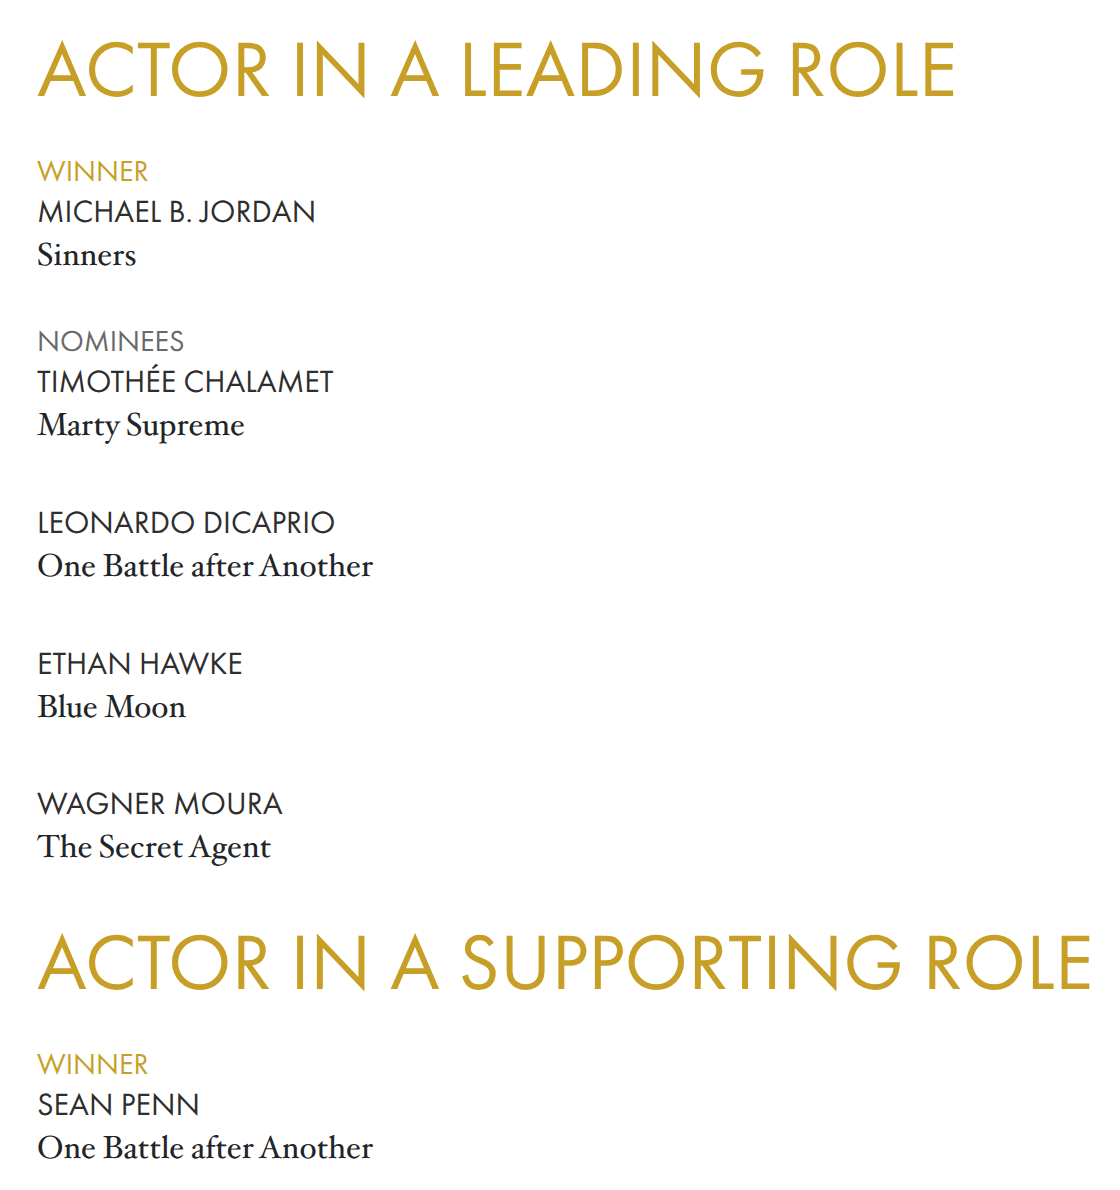
\includegraphics[width=1120\unitlength]{oscars_card.png}};
  \draw[black!25] (0,0) rectangle (1120,1190);
  \node[small marker] at (992,67) {3};                % the card's name
  \draw[marker thin lead] (156,172) -- (318,152);     % Winner
  \node[small marker] at (345,150) {5};
  \node[small marker] at (360,212) {6};               % the person
  \draw[marker thin lead] (144,257) -- (318,273);     % the film
  \node[small marker] at (345,275) {7};
  \draw[marker brace] (405,156) -- (405,280);         % one honoree
  \node[small marker] at (462,218) {4};
  \draw[marker brace] (1040,28) -- (1040,871);        % one card
  \node[small marker] at (1078,450) {2};
  % the area around all 24 cards; it continues below the picture
  \draw[tab-blue,line width=0.9pt] (1106,28) -- (1118,28) -- (1118,1150);
  \draw[tab-blue,line width=0.9pt,-latex] (1118,1150) -- (1118,1205);
  \node[small marker] at (1150,620) {1};
\end{tikzpicture}
\end{document}
